\documentclass[11pt]{report}

\usepackage[a4paper,margin=1in]{geometry}
\usepackage[T1]{fontenc}
\usepackage[utf8]{inputenc}
\usepackage{lmodern}
\usepackage{microtype}
\usepackage{setspace}
\usepackage{mathtools,amssymb,amsthm,bm}
\usepackage{array}
\usepackage{booktabs}
\usepackage{longtable}
\usepackage{graphicx}
\usepackage{float}
\usepackage{enumitem}
\usepackage{xcolor}
\usepackage{xurl}
\usepackage[plainpages=false,pdfpagelabels]{hyperref}
\usepackage{bookmark}
\usepackage{caption}
\usepackage{fancyhdr}
\usepackage{listings}
\usepackage{titlesec}
\usepackage{tocloft}

\hypersetup{
  colorlinks=true,
  linkcolor=blue!50!black,
  urlcolor=blue!50!black,
  citecolor=blue!50!black,
  pdftitle={Graviton Basis Toolkit Report},
  pdfauthor={Prepared from graviton basis toolkit wl},
  pdfsubject={Graviton basis reduction modulo integration by parts and field redefinitions}
}

\setstretch{1.06}
\setlength{\headheight}{14pt}
\setlength{\emergencystretch}{2em}
\allowdisplaybreaks[2]
\setcounter{tocdepth}{2}
\captionsetup{font=small,labelfont=bf}
\numberwithin{equation}{chapter}

\pagestyle{fancy}
\fancyhf{}
\fancyhead[L]{Graviton Basis Toolkit Report}
\fancyhead[R]{\thepage}
\fancypagestyle{plain}{
  \fancyhf{}
  \fancyhead[L]{Graviton Basis Toolkit Report}
  \fancyhead[R]{\thepage}
}

\lstdefinestyle{mma}{
  basicstyle=\ttfamily\small,
  breaklines=true,
  columns=fullflexible,
  keepspaces=true,
  frame=single,
  rulecolor=\color{black!25},
  backgroundcolor=\color{black!2},
  showstringspaces=false
}

\titleformat{\chapter}[display]
  {\bfseries\Large}
  {\filright\Large\chaptername~\thechapter}
  {1ex}
  {\titlerule\vspace{1ex}\filright}

\newtheorem{definition}{Definition}[chapter]
\newtheorem{proposition}[definition]{Proposition}
\newtheorem{remark}[definition]{Remark}

\newcommand{\toolkit}{\texttt{graviton\_basis\_toolkit.wl}}
\newcommand{\reportdata}{\texttt{graviton\_basis\_toolkit\_comprehensive\_report\_data.wl}}
\newcommand{\validationdata}{\texttt{graviton\_basis\_toolkit\_validation\_output.wl}}
\newcommand{\Lag}{\mathcal{L}}

\newcommand{\Vspace}[2]{\mathcal{V}_{#1,#2}}
\newcommand{\Tspace}[2]{\mathcal{T}_{#1,#2}}
\newcommand{\Qspace}[2]{\mathcal{Q}_{#1,#2}}
\newcommand{\Rspace}[2]{\mathcal{R}_{#1,#2}}
\newcommand{\Pspace}[2]{\mathcal{P}_{#1,#2}}
\newcommand{\Dspace}[2]{\mathcal{D}_{#1,#2}}
\newcommand{\Comp}{\operatorname{Comp}}
\newcommand{\Can}{\operatorname{Can}}
\newcommand{\Contr}{\operatorname{Contr}}
\newcommand{\Span}{\operatorname{span}}
\newcommand{\Ker}{\operatorname{Ker}}
\newcommand{\Image}{\operatorname{Im}}
\newcommand{\Rank}{\operatorname{rank}}
\newcommand{\ProjIBP}{\Pi_{\mathrm{IBP}}}
\newcommand{\Projphys}{\Pi_{\mathrm{phys}}}
\newcommand{\LagFP}{\mathcal{L}_{\mathrm{FP}}^{(2)}}
\newcommand{\Euler}{\mathcal{E}}
\newcommand{\Raw}{\mathrm{raw}}
\newcommand{\IBP}{\mathrm{IBP}}
\newcommand{\Phys}{\mathrm{phys}}
\newcommand{\FieldRed}{\mathrm{FR}}

\begin{document}

\hypersetup{pageanchor=false}
\begin{titlepage}
\thispagestyle{empty}
\centering
\vspace*{2.5cm}
{\Huge\bfseries Graviton Basis Toolkit Report\par}
\vspace{0.9cm}
{\Large Mathematical Background, Software Reference, Validation,\\ and a Worked Reduction Example\par}
\vspace{1.8cm}
{\large Prepared from \toolkit\par}
\vspace{0.4cm}
{\large March 2026\par}
\vfill
{\large
Arbitrary-dimension linearized graviton operator bases with\\
integration-by-parts reduction, Fierz--Pauli field redefinitions,\\
sector-level caching, and direct Lagrangian reduction.\par}
\vfill
\end{titlepage}

\clearpage
\hypersetup{pageanchor=true}
\pagenumbering{roman}

\chapter*{Abstract}
\addcontentsline{toc}{chapter}{Abstract}

This report documents the current graviton-basis reduction toolkit.
The implementation analyzed here is the Wolfram Language source file \toolkit.
The toolkit takes local scalar operators built from a linearized graviton \(h_{\mu\nu}\) and flat-space derivatives,
construct the sector basis, and reduce that basis modulo integration by parts and, for interaction sectors,
modulo the image of Fierz--Pauli field redefinitions.

The report is written in the style of a technical paper rather than a notebook manual.
It starts from the mathematical formulation of the quotient problem,
develops the sector-local linear algebra used by the code,
explains the software architecture and user-facing entry points,
validates the implementation on explicit equation-of-motion images,
and finishes with a fully worked nontrivial reduction example whose input contains both kinds of redundancy
while leaving a nonzero physical representative after the reduction.

\tableofcontents
\clearpage
\pagenumbering{arabic}

\chapter{Purpose and Scope}

The toolkit in \toolkit\ automates the classification of local scalar graviton operators on flat space.
More precisely, given the symmetric rank-2 field \(h_{\mu\nu}\), the code constructs local scalar operators built from:
\begin{itemize}
\item \(n_h\) copies of \(h_{\mu\nu}\),
\item \(N_\partial\) partial derivatives,
\item the flat metric \(\eta_{\mu\nu}\),
\end{itemize}
and then performs two quotient operations:
\begin{enumerate}[label=\arabic*.]
\item quotient by integration by parts (IBP),
\item quotient by the image of local field redefinitions acting through the quadratic Fierz--Pauli action.
\end{enumerate}

The organizational principle of the implementation is the sector grading
\begin{equation}
  D = n_h + N_\partial,
  \label{eq:total_dimension}
\end{equation}
where \(D\) is the total engineering dimension in the counting convention used by the code.
Because both the IBP quotient and the field-redefinition image preserve the ordered pair \((n_h,N_\partial)\),
the full problem decomposes into finite-dimensional linear-algebra problems on independent sectors.

The present toolkit goes beyond the original one-sector notebook workflow in four ways:
\begin{itemize}
\item it generates raw graviton bases for arbitrary sectors;
\item it computes the IBP quotient in a fully sector-local form;
\item it computes the field-redefinition quotient in the same sector-local language;
\item it provides a direct reducer for explicit Lagrangians, not only basis counts.
\end{itemize}

The purpose of this report is therefore broader than a user guide.
It is meant to serve simultaneously as:
\begin{enumerate}[label=\alph*.]
\item a mathematical explanation of the quotient spaces being computed;
\item a reference for the code architecture and public API;
\item a validation record tied to explicit equations and explicit computed outputs;
\item a worked example showing an actual nontrivial Lagrangian reduction end to end.
\end{enumerate}

\chapter{Mathematical Framework}

\section{Sector spaces}

\begin{definition}
For fixed nonnegative integers \((n_h,N_\partial)\), define \(\Vspace{n_h}{N_\partial}\) to be the vector space of local scalar expressions built from:
\begin{enumerate}[label=\roman*.]
\item \(n_h\) copies of the symmetric field \(h_{\mu\nu}\),
\item \(N_\partial\) flat derivatives,
\item the flat metric \(\eta_{\mu\nu}\),
\end{enumerate}
modulo canonical tensor identities and index symmetries.
\end{definition}

The toolkit works sector by sector in these spaces.
The finiteness of the computation in each sector relies on two observations:
\begin{enumerate}[label=\roman*.]
\item the number of ordered derivative placements at fixed \((n_h,N_\partial)\) is finite;
\item the set of independent Lorentz contractions of a fixed seed monomial is finite.
\end{enumerate}

The derivative-placement data are encoded by ordered compositions
\begin{equation}
  \Comp(N_\partial,n_h)
  :=
  \left\{
    (k_1,\dots,k_{n_h}) \in \mathbb{Z}_{\ge 0}^{\,n_h}
    \;\middle|\;
    \sum_{i=1}^{n_h} k_i = N_\partial
  \right\}.
  \label{eq:composition_set}
\end{equation}
For each \(\bm{k}=(k_1,\dots,k_{n_h}) \in \Comp(N_\partial,n_h)\), the corresponding seed monomial is
\begin{equation}
  M_{\bm{k}}
  :=
  \prod_{i=1}^{n_h} \partial^{k_i} h.
  \label{eq:seed_monomial}
\end{equation}
The notation in \eqref{eq:seed_monomial} is schematic: the actual code keeps all indices explicit and uses xAct to canonicalize them.

\section{Raw basis generation}

The raw sector basis is generated from the ordered compositions by taking all scalar contractions and canonicalizing the result:
\begin{equation}
  \mathcal{B}^{\Raw}_{n_h,N_\partial}
  :=
  \Can\!\left(
    \bigcup_{\bm{k}\in \Comp(N_\partial,n_h)}
    \Contr(M_{\bm{k}})
  \right).
  \label{eq:raw_basis}
\end{equation}
Equation \eqref{eq:raw_basis} is the mathematical content of the code path
\begin{center}
\texttt{CompositionList \(\to\) RawScalarMonomials \(\to\) AllContractions \(\to\) canonExpr}.
\end{center}

Two remarks are important here.
First, the derivative compositions are ordered, not unordered.
This matters because distinct derivative placements can become equivalent only after canonicalization and/or IBP;
they are not equivalent at the seed stage.
Second, the code skips odd-\(N_\partial\) scalar sectors because in the present flat-space setup those sectors have no fully contracted scalar monomials.

For the cubic two-derivative sector one has
\begin{equation}
  (n_h,N_\partial)=(3,2),
  \qquad
  \Vspace{3}{2}
  =
  \Span\!\left\{
    h(\partial h)(\partial h),
    \;
    hh(\partial\partial h)
  \right\}.
  \label{eq:v32_schematic}
\end{equation}
The raw basis generated by the code contains both schematic classes in \eqref{eq:v32_schematic}.

\begin{figure}[tbp]
  \centering
  
\includegraphics[width=0.82\textwidth,height=0.30\textheight,keepaspectratio]{paper_assets/basis_pipeline.pdf}
  \caption{Raw basis generation followed by the two quotient operations.}
  \label{fig:basis_pipeline}
\end{figure}

\section{IBP as a kernel quotient}

Let \(\Tspace{n_h}{N_\partial} \subset \Vspace{n_h}{N_\partial}\) denote the subspace of total derivatives.
The first quotient space is
\begin{equation}
  \Qspace{n_h}{N_\partial}
  :=
  \Vspace{n_h}{N_\partial} / \Tspace{n_h}{N_\partial}.
  \label{eq:ibp_quotient}
\end{equation}

The reduction criterion used by the toolkit is the Euler-operator criterion:
\begin{proposition}
For a local scalar density \(X\),
\begin{equation}
  X \in \Tspace{n_h}{N_\partial}
  \qquad \Longleftrightarrow \qquad
  \Euler(X) := \frac{\delta X}{\delta h_{\mu\nu}} = 0.
  \label{eq:euler_criterion}
\end{equation}
\end{proposition}

Operationally, if
\begin{equation}
  \mathcal{B}^{\Raw}_{n_h,N_\partial}
  =
  \left(
    O_1,\dots,O_r
  \right),
\end{equation}
the code introduces an ansatz
\begin{equation}
  X(\bm{c})
  :=
  \sum_{i=1}^{r} c_i O_i
  \label{eq:ibp_ansatz}
\end{equation}
and solves
\begin{equation}
  \Euler(X(\bm{c})) = 0
  \label{eq:ibp_equations}
\end{equation}
for the coefficients \(\bm{c}=(c_1,\dots,c_r)\).
The solution space of \eqref{eq:ibp_equations} yields the IBP relation matrix, whose row space is the subspace of raw-basis combinations that vanish in \(\Qspace{n_h}{N_\partial}\).

If \(M_{\IBP}\) denotes this relation matrix, then the IBP quotient basis
\(
\mathcal{B}^{\IBP}_{n_h,N_\partial}
\)
is obtained by deleting pivot columns.
At the level of dimensions,
\begin{equation}
  \dim \Qspace{n_h}{N_\partial}
  =
  \dim \Vspace{n_h}{N_\partial}
  -
  \Rank M_{\IBP}.
  \label{eq:ibp_dimension_formula}
\end{equation}

\section{Field redefinitions as an image quotient}

The quadratic Fierz--Pauli Lagrangian is
\begin{equation}
\begin{aligned}
\LagFP
&=
-
\frac{1}{2}\,
\partial_\rho h_{\mu\nu}\partial^\rho h^{\mu\nu}
+
\partial_\mu h^{\mu\nu}\partial^\rho h_{\rho\nu}
-
\partial_\mu h^{\mu\nu}\partial_\nu h
+
\frac{1}{2}\,
\partial_\rho h\,\partial^\rho h .
\end{aligned}
\label{eq:fierz_pauli}
\end{equation}

For a local symmetric rank-2 tensor \(\Delta h_{\mu\nu}\), the linearized variation is
\begin{equation}
  \delta \LagFP
  =
  E_{\mathrm{FP}}^{\mu\nu}\,\Delta h_{\mu\nu}
  +
  \partial_\rho K^\rho.
  \label{eq:fp_variation}
\end{equation}
Hence all such images are redundant modulo IBP.

Define the source rank-2 space by
\begin{equation}
  \Dspace{n_h-1}{N_\partial-2}
  :=
  \left\{
    \begin{array}{c}
      \text{symmetric local rank-2 tensors} \\
      \text{with \(n_h-1\) gravitons and \(N_\partial-2\) derivatives}
    \end{array}
  \right\}.
  \label{eq:rank2_space}
\end{equation}
The corresponding field-redefinition map into the IBP quotient is
\begin{equation}
  F_{n_h,N_\partial} :
  \Dspace{n_h-1}{N_\partial-2}
  \longrightarrow
  \Qspace{n_h}{N_\partial},
  \qquad
  F_{n_h,N_\partial}(\Delta h)
  :=
  \ProjIBP\!\left(
    \left.
    \frac{d}{d\lambda}
    \LagFP[h+\lambda \Delta h]
    \right|_{\lambda=0}
  \right).
  \label{eq:field_redefinition_map}
\end{equation}

Its image is
\begin{equation}
  \Rspace{n_h}{N_\partial}
  :=
  \Image F_{n_h,N_\partial}
  \subset
  \Qspace{n_h}{N_\partial}.
  \label{eq:image_space}
\end{equation}
For interaction sectors, the final quotient space classified by the toolkit is
\begin{equation}
  \Pspace{n_h}{N_\partial}
  :=
  \Qspace{n_h}{N_\partial} / \Rspace{n_h}{N_\partial}.
  \label{eq:physical_quotient}
\end{equation}

\begin{proposition}
For \(n_h \ge 3\),
\begin{equation}
  \dim \Pspace{n_h}{N_\partial}
  =
  \dim \Qspace{n_h}{N_\partial}
  -
  \Rank I_{n_h,N_\partial},
  \label{eq:physical_dimension_formula}
\end{equation}
where \(I_{n_h,N_\partial}\) is the matrix whose independent rows are the coordinate vectors of the projected field-redefinition images in the IBP basis.
\end{proposition}

\begin{figure}[tbp]
  \centering
  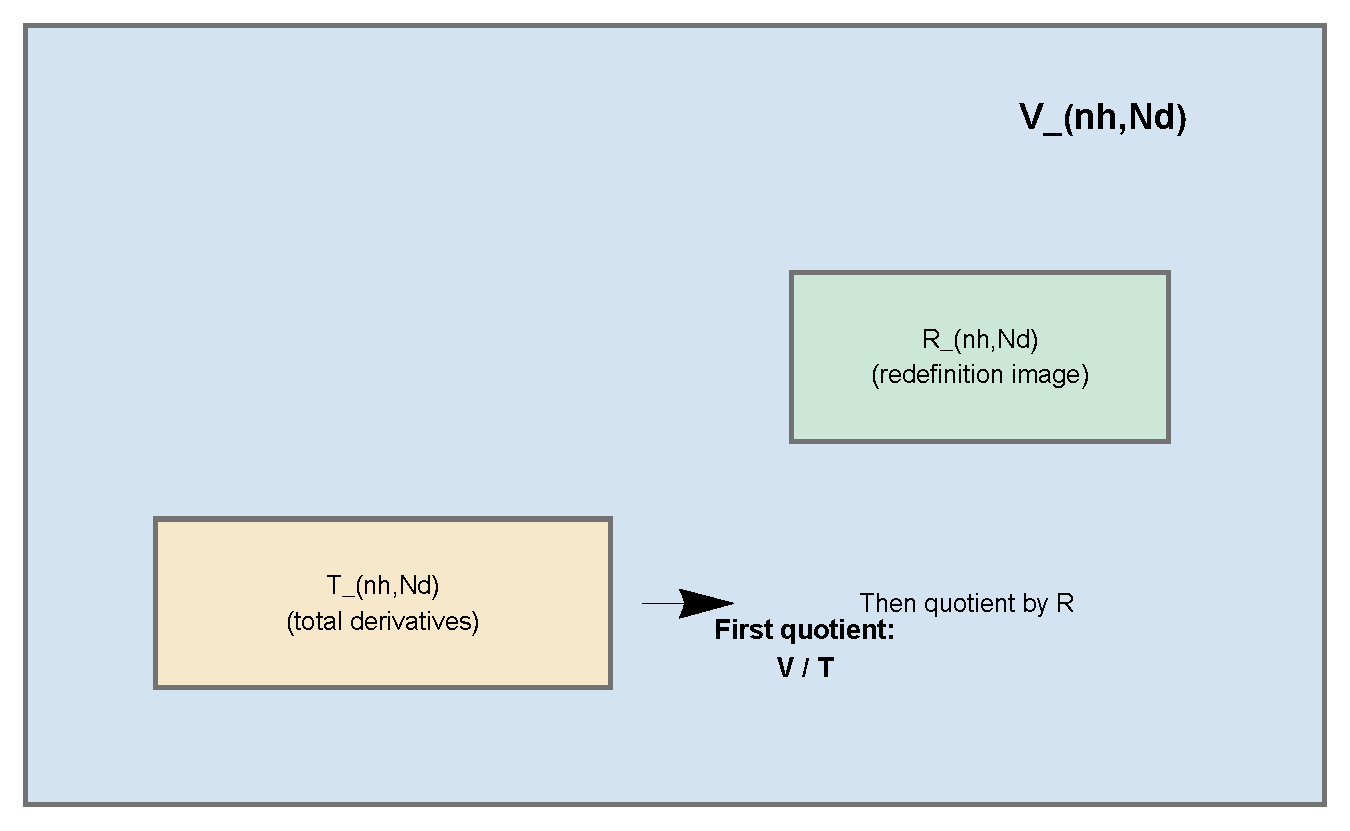
\includegraphics[width=0.76\textwidth,height=0.30\textheight,keepaspectratio]{paper_assets/quotient_space.pdf}
  \caption{The quotient-space structure of the algorithm.}
  \label{fig:quotient_space}
\end{figure}

\section{Coordinate-level reduction formula}

Suppose the IBP quotient basis of a target sector is
\begin{equation}
  \mathcal{B}^{\IBP}_{n_h,N_\partial}
  =
  (B_1,\dots,B_q).
\end{equation}
Any projected expression \(X\in \Qspace{n_h}{N_\partial}\) can be written as
\begin{equation}
  X = \sum_{j=1}^{q} q_j B_j,
  \qquad
  \bm{q}=(q_1,\dots,q_q).
  \label{eq:ibp_coordinates}
\end{equation}

Let the independent field-redefinition image vectors be
\begin{equation}
  \bm{i}_1,\dots,\bm{i}_m \in \mathbb{K}^{q},
  \label{eq:image_vectors}
\end{equation}
assembled as the rows of a matrix \(I_{\mathrm{ind}}\).
Let \(p\subset\{1,\dots,q\}\) denote the corresponding pivot columns.
The coefficient vector \(\bm{\alpha}\) of the removable image component is determined by
\begin{equation}
  \sum_{a=1}^{m} \alpha_a (\bm{i}_a)_{p}
  =
  \bm{q}_{p}.
  \label{eq:image_coeff_equation}
\end{equation}
The reduced IBP coordinates are then
\begin{equation}
  \bm{q}^{\,\mathrm{red}}
  =
  \bm{q}
  -
  \sum_{a=1}^{m} \alpha_a \bm{i}_a.
  \label{eq:reduced_ibp_coords}
\end{equation}
Finally, deleting the pivot entries yields the physical coordinates
\begin{equation}
  \bm{q}^{\,\Phys}
  =
  \operatorname{Delete}_{p}
  \bigl(
    \bm{q}^{\,\mathrm{red}}
  \bigr).
  \label{eq:physical_coords}
\end{equation}
Equations \eqref{eq:image_coeff_equation}--\eqref{eq:physical_coords} are implemented directly by the helper
\texttt{ReduceCoordinatesModulo\-Redef}.

\section{Quadratic sectors and gauge invariance}

The current convention in the toolkit is
\begin{equation}
  n_h < 3 \; \Longrightarrow \; \text{reduce modulo IBP only}.
  \label{eq:quadratic_convention}
\end{equation}
This is deliberate.
At quadratic order, a linear redefinition can act directly on the kinetic operator itself, so quotienting by those directions is not the desired classification if one wants to retain a meaningful notion of the quadratic action.

The toolkit also does not automatically impose linearized diffeomorphism invariance.
Its quotients are by:
\begin{equation}
  \text{IBP}
  \qquad \text{and} \qquad
  \text{Fierz--Pauli field redefinitions},
\end{equation}
not by gauge symmetry.
Gauge invariance is therefore an additional condition one may impose after the quotient basis has been constructed.
The linearized gauge transformation is
\begin{equation}
  \delta_\xi h_{\mu\nu}
  =
  \partial_\mu \xi_\nu + \partial_\nu \xi_\mu .
  \label{eq:linear_gauge_transform}
\end{equation}
From it one obtains the standard linearized curvatures
\begin{align}
  R^{(1)}_{\mu\nu\rho\sigma}
  &=
  \tfrac{1}{2}
  \bigl(
    \partial_\rho \partial_\nu h_{\mu\sigma}
    + \partial_\sigma \partial_\mu h_{\nu\rho}
    - \partial_\sigma \partial_\nu h_{\mu\rho}
    - \partial_\rho \partial_\mu h_{\nu\sigma}
  \bigr),
  \label{eq:linear_riemann}
  \\
  R^{(1)}_{\mu\nu}
  &=
  \partial_\rho \partial_{(\mu} h_{\nu)}{}^\rho
  - \tfrac{1}{2}\Box h_{\mu\nu}
  - \tfrac{1}{2}\partial_\mu \partial_\nu h,
  \label{eq:linear_ricci}
  \\
  R^{(1)}
  &=
  \partial_\mu \partial_\nu h^{\mu\nu} - \Box h.
  \label{eq:linear_scalar_curvature}
\end{align}
Accordingly, the gauge-invariant subspace of \(\Vspace{2}{4}\) is spanned by quadratic curvature combinations such as
\begin{equation}
  \bigl(R^{(1)}\bigr)^2,
  \qquad
  R^{(1)}_{\mu\nu} R^{(1)\mu\nu},
  \qquad
  R^{(1)}_{\mu\nu\rho\sigma} R^{(1)\mu\nu\rho\sigma},
  \label{eq:curvature_squared_space}
\end{equation}
subject in four dimensions to the Gauss--Bonnet total-derivative relation
\begin{equation}
  R^{(1)}_{\mu\nu\rho\sigma} R^{(1)\mu\nu\rho\sigma}
  - 4 R^{(1)}_{\mu\nu} R^{(1)\mu\nu}
  + \bigl(R^{(1)}\bigr)^2
  \in
  \Tspace{2}{4}.
  \label{eq:gauss_bonnet_linearized}
\end{equation}
This explains why a quadratic four-derivative basis modulo IBP is larger than the curvature-squared subspace:
the former is an off-shell operator space, whereas the latter is the gauge-invariant subspace inside it.

\chapter{Software Architecture and Usage}

\section{Implementation blocks}

The file \toolkit\ is organized around a compact set of high-level blocks.
The practical role of the public entry points is summarized in Table~\ref{tab:functions}.

\begin{table}[tbp]
\centering
\caption{Main public functions in the toolkit.}
\label{tab:functions}
{\small
\begin{tabular}{>{\raggedright\arraybackslash}p{0.35\textwidth} >{\raggedright\arraybackslash}p{0.52\textwidth}}
\toprule
Function & Purpose \\
\midrule
\texttt{RunBasisComputation} & Loop over sectors, compute or load sector data, and return a summary association. \\
\texttt{ComputeSectorData} & Execute the raw-basis, IBP, and field-redefinition pipeline for one sector. \\
\texttt{RawBasisOfSector} & Extract the raw scalar basis from a stored sector result. \\
\texttt{IBPBasisOfSector} & Extract the basis modulo total derivatives. \\
\texttt{PhysicalBasisOfSector} & Extract the final interaction-sector basis after removing the redefinition image. \\
\texttt{RedefinitionRulesOfSector} & Return independent field redefinitions and their images in the IBP basis. \\
\texttt{ReduceSectorLagrangian} & Reduce a single-sector Lagrangian modulo IBP and field redefinitions. \\
\texttt{ReduceLagrangian} & Split a general Lagrangian by sector and reduce each sector automatically. \\
\bottomrule
\end{tabular}
}
\end{table}

\section{Canonicalization and data flow}

The core normal-form map in the code is \texttt{canonExpr}.
Its role is mathematically straightforward:
\begin{enumerate}[label=\arabic*.]
\item expand the expression;
\item contract the flat metric;
\item canonicalize tensor symmetries;
\item sort nested derivatives;
\item canonicalize again;
\item collect tensor structures.
\end{enumerate}
The second canonicalization pass is essential for making the Euler-operator test reliable on expanded total derivatives.

\begin{figure}[tbp]
  \centering
  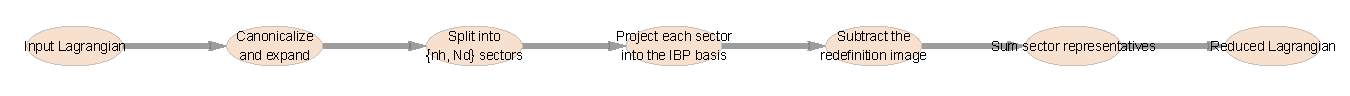
\includegraphics[width=0.82\textwidth,height=0.30\textheight,keepaspectratio]{paper_assets/reducer_pipeline.pdf}
  \caption{Logical flow of the Lagrangian reducer.}
  \label{fig:reducer_pipeline}
\end{figure}

\section{User-facing workflow}

A standard run up to mass dimension five is
\begin{lstlisting}[style=mma]
Get["graviton_basis_toolkit.wl"];

res = RunBasisComputation[
  "MaxDimension" -> 5,
  "CacheDirectory" -> FileNameJoin[{Directory[], "basis_cache"}],
  "UseCache" -> True,
  "Verbose" -> True
];
\end{lstlisting}

Typical inspection calls are
\begin{lstlisting}[style=mma]
RawBasisOfSector[res, 3, 2]
IBPBasisOfSector[res, 3, 2]
PhysicalBasisOfSector[res, 3, 2]
RedefinitionRulesOfSector[res, 3, 2]
\end{lstlisting}

To reduce an explicit Lagrangian:
\begin{lstlisting}[style=mma]
red = ReduceLagrangian[lag,
  "CacheDirectory" -> FileNameJoin[{Directory[], "basis_cache"}],
  "UseCache" -> True
];

red["ReducedExpression"]
\end{lstlisting}

\section{Sector summary used in this report}

Table~\ref{tab:summary} records the current validated counts used in the present report.

\begin{table}[tbp]
\centering
\caption{Current sector counts used in the report.}
\label{tab:summary}
\begin{tabular}{ccccc}
\toprule
Sector & RawCount & IBPCount & RedefRank & PhysicalCount \\
\midrule
\((1,2)\) & 2  & 0  & 0 & 0  \\
\((2,2)\) & 10 & 4  & 0 & 4  \\
\((2,4)\) & 30 & 5  & 0 & 5  \\
\((3,2)\) & 28 & 14 & 4 & 10 \\
\bottomrule
\end{tabular}
\end{table}

The \((3,2)\) sector is the first interaction sector and therefore the first one in which the field-redefinition quotient is nontrivial.
That is why it is also the sector chosen for the detailed validation and the worked example below.

\chapter{Validation}

\section{Validation philosophy}

The cleanest test of the image quotient is to evaluate the reducer on expressions that are known by construction to lie in \(\Rspace{n_h}{N_\partial}\).
By \eqref{eq:fp_variation}, such an expression is an equation-of-motion term up to a total derivative, so its reduced representative must vanish.

\begin{figure}[tbp]
  \centering
  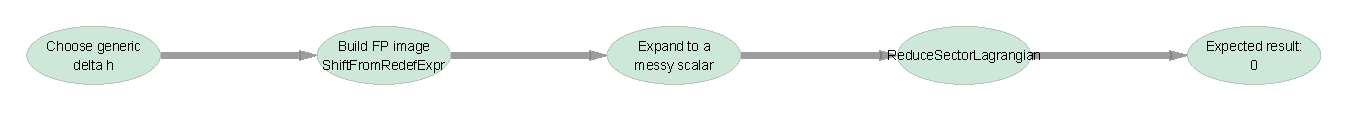
\includegraphics[width=0.8\textwidth,height=0.30\textheight,keepaspectratio]{paper_assets/validation_pipeline.pdf}
  \caption{Validation strategy used in the report.}
  \label{fig:validation_pipeline}
\end{figure}

\section{Detailed validation in sector (3,2)}

Choose coefficients
\begin{equation}
  \bm{\alpha}^{(32)} = (7,-11,13,-17)
  \label{eq:validation_alpha}
\end{equation}
in the independent rank-2 basis of source sector \((2,0)\).
The corresponding redefinition is
\begin{equation}
  \Delta h_{\mu\nu}^{(32)}
  =
  \sum_{a=1}^{4}
  \alpha^{(32)}_{a}\,
  \Delta^{(a)}_{\mu\nu}.
  \label{eq:validation_delta}
\end{equation}
In Mathematica notation, this is
\begin{lstlisting}[style=mma]
7*h[u, z$28894]*h[v, -z$28894]
- 11*h[u, v]*h[z$28894, -z$28894]
+ 13*eta[u, v]*h[-z$28894, -z$28943]*h[z$28894, z$28943]
- 17*eta[u, v]*h[z$28894, -z$28894]*h[z$28943, -z$28943]
\end{lstlisting}

Applying the Fierz--Pauli variation and expanding gives a 12-term scalar expression in the target sector \((3,2)\):
\begin{lstlisting}[style=mma]
11*h[a, b]*PD[-a][h[c, -c]]*PD[-b][h[z$28894, -z$28894]]
- 29*h[a, b]*PD[-b][h[z$28894, -z$28894]]*PD[-c][h[-a, c]]
- 7*h[a, b]*PD[-b][h[-a, c]]*PD[-c][h[z$28894, -z$28894]]
+ 77*h[a, b]*PD[-c][h[z$28894, -z$28894]]*PD[c][h[-a, -b]]
- 90*h[a, -a]*PD[-c][h[z$28894, -z$28894]]*PD[c][h[b, -b]]
+ 14*h[a, b]*PD[-c][h[-a, c]]*PD[-z$28894][h[-b, z$28894]]
+ 14*h[a, b]*PD[-b][h[-a, c]]*PD[-z$28894][h[-c, z$28894]]
- 22*h[a, -a]*PD[-b][h[b, c]]*PD[-z$28894][h[-c, z$28894]]
- 66*h[a, b]*PD[c][h[-a, -b]]*PD[-z$28894][h[-c, z$28894]]
+ 101*h[a, -a]*PD[c][h[b, -b]]*PD[-z$28894][h[-c, z$28894]]
- 14*h[a, b]*PD[-z$28894][h[-b, -c]]*PD[z$28894][h[-a, c]]
+ 11*h[a, -a]*PD[-z$28894][h[-b, -c]]*PD[z$28894][h[b, c]]
\end{lstlisting}

The image-coordinate test is then
\begin{equation}
  \bm{q}^{(32)}_{\IBP}
  =
  \sum_{a=1}^{4} \alpha^{(32)}_{a}\,\bm{i}_{a}^{(32)},
  \label{eq:validation_image_decomposition}
\end{equation}
with the computed projected IBP coordinates
\begin{equation}
  \bm{q}^{(32)}_{\IBP}
  =
  \{0,11,-36,77,-90,0,7,-66,101,14,14,-14,-29,11\}.
  \label{eq:validation_ibp_coords}
\end{equation}
The reducer recovers exactly the same image coefficients as in \eqref{eq:validation_alpha}:
\begin{equation}
  \bm{\alpha}^{(32)}_{\mathrm{recovered}}
  =
  \{7,-11,13,-17\}.
  \label{eq:validation_recovered_alpha}
\end{equation}
After subtracting the image component, the physical coordinates are
\begin{equation}
  \bm{q}^{(32)}_{\Phys}
  =
  \{0,0,0,0,0,0,0,0,0,0\}.
  \label{eq:validation_zero_phys}
\end{equation}
Accordingly, the reduced representative is
\begin{lstlisting}[style=mma]
0
\end{lstlisting}
exactly as required by the quotient \(\Pspace{3}{2}\).

\section{Stored stress test in sector (3,4)}

The \((3,2)\) test checks the first nontrivial interaction sector.
The stronger stored test uses source sector \((2,2)\) and target sector \((3,4)\).
There, the source redefinition basis has 33 independent directions and its expanded image in the target sector contains 240 scalar terms.
The reducer again returns zero.

Table~\ref{tab:validation} summarizes the stored validation results.

\begin{table}[tbp]
\centering
\caption{Stored validation results from \validationdata.}
\label{tab:validation}
{\small
\begin{tabular}{@{}ccccccc@{}}
\toprule
Sector & \(\dim \mathcal{Q}\) & \(\Rank F\) & \(\dim \mathcal{P}\) & \(\dim \mathcal{D}\) & Terms & Zero? \\
\midrule
\((3,2)\) & 14 & 4  & 10 & 4  & 18  & Yes \\
\((3,4)\) & 64 & 33 & 31 & 33 & 240 & Yes \\
\bottomrule
\end{tabular}
}
\end{table}

\section{Why these tests are nontrivial}

The validation expressions are not fed to the reducer in a disguised symbolic form such as \(E_{\mathrm{FP}}^{\mu\nu}\Delta h_{\mu\nu}\).
They are first expanded into explicit scalar monomials with many terms and non-obvious cancellations.
Consequently, the zero result is not tautological:
it certifies that the canonicalization, IBP projection, and image subtraction are cooperating correctly.

\chapter{Worked Example: A Nontrivial Reduction}

\section{Construction of the input Lagrangian}

We again work in the target sector \((3,2)\), but now the aim is different:
the reduced answer should be nonzero.
To achieve this, define
\begin{equation}
  \Lag_{\mathrm{in}}
  =
  \Lag_{\Phys}
  +
  4\,\Lag_{\IBP}
  +
  \Lag_{\FieldRed},
  \label{eq:worked_input_decomposition}
\end{equation}
where:
\begin{itemize}
\item \(\Lag_{\Phys}\) is chosen directly in the physical basis,
\item \(\Lag_{\IBP}\) is chosen from the explicit IBP-relation list,
\item \(\Lag_{\FieldRed}\) is chosen from the image of the Fierz--Pauli variation.
\end{itemize}

The physical part is
\begin{equation}
  \Lag_{\Phys}
  =
  2\,h^{ab}\,\partial_a h^{cd}\,\partial_b h_{cd}
  -
  3\,h^{ab}\,\partial_b h_{a}{}^{c}\,\partial^{d} h_{cd},
  \label{eq:worked_physical_part}
\end{equation}
which in Mathematica notation is
\begin{lstlisting}[style=mma]
2*h[a, b]*PD[-a][h[c, d]]*PD[-b][h[-c, -d]]
- 3*h[a, b]*PD[-b][h[-a, c]]*PD[-d][h[-c, d]]
\end{lstlisting}
and corresponds to the target physical-coordinate vector
\begin{equation}
  \bm{p}_{\Phys}
  =
  \{2,-3,0,0,0,0,0,0,0,0\}.
  \label{eq:worked_phys_coords}
\end{equation}

The chosen IBP-trivial contribution is
\begin{lstlisting}[style=mma]
h[a, b]*PD[-b][h[d, -d]]*PD[-c][h[-a, c]]
+ h[a, b]*PD[-b][h[-a, c]]*PD[-c][h[d, -d]]
+ h[-a, c]*h[a, b]*PD[-c][PD[-b][h[d, -d]]]
\end{lstlisting}
which vanishes in \(\Qspace{3}{2}\) by \eqref{eq:euler_criterion}.

The field-redefinition image is chosen with coefficients
\begin{equation}
  \bm{\alpha}_{\FieldRed}
  =
  \{5,-7,11,-13\}.
  \label{eq:worked_alpha}
\end{equation}
Its expanded Mathematica expression is
\begin{lstlisting}[style=mma]
7*h[a, b]*PD[-a][h[c, -c]]*PD[-b][h[z$28894, -z$28894]]
- 19*h[a, b]*PD[-b][h[z$28894, -z$28894]]*PD[-c][h[-a, c]]
- 5*h[a, b]*PD[-b][h[-a, c]]*PD[-c][h[z$28894, -z$28894]]
+ 61*h[a, b]*PD[-c][h[z$28894, -z$28894]]*PD[c][h[-a, -b]]
- 66*h[a, -a]*PD[-c][h[z$28894, -z$28894]]*PD[c][h[b, -b]]
+ 10*h[a, b]*PD[-c][h[-a, c]]*PD[-z$28894][h[-b, z$28894]]
+ 10*h[a, b]*PD[-b][h[-a, c]]*PD[-z$28894][h[-c, z$28894]]
- 14*h[a, -a]*PD[-b][h[b, c]]*PD[-z$28894][h[-c, z$28894]]
- 54*h[a, b]*PD[c][h[-a, -b]]*PD[-z$28894][h[-c, z$28894]]
+ 73*h[a, -a]*PD[c][h[b, -b]]*PD[-z$28894][h[-c, z$28894]]
- 10*h[a, b]*PD[-z$28894][h[-b, -c]]*PD[z$28894][h[-a, c]]
+ 7*h[a, -a]*PD[-z$28894][h[-b, -c]]*PD[z$28894][h[b, c]]
\end{lstlisting}

Combining the three pieces gives the 14-term input Lagrangian
\begin{lstlisting}[style=mma]
2*h[a, b]*PD[-a][h[c, d]]*PD[-b][h[-c, -d]]
+ 7*h[a, b]*PD[-a][h[c, -c]]*PD[-b][h[d, -d]]
- 15*h[a, b]*PD[-b][h[d, -d]]*PD[-c][h[-a, c]]
- h[a, b]*PD[-b][h[-a, c]]*PD[-c][h[d, -d]]
+ 4*h[-a, c]*h[a, b]*PD[-c][PD[-b][h[d, -d]]]
+ 61*h[a, b]*PD[-c][h[d, -d]]*PD[c][h[-a, -b]]
- 66*h[a, -a]*PD[-c][h[d, -d]]*PD[c][h[b, -b]]
+ 10*h[a, b]*PD[-c][h[-a, c]]*PD[-d][h[-b, d]]
+ 7*h[a, b]*PD[-b][h[-a, c]]*PD[-d][h[-c, d]]
- 14*h[a, -a]*PD[-b][h[b, c]]*PD[-d][h[-c, d]]
- 54*h[a, b]*PD[c][h[-a, -b]]*PD[-d][h[-c, d]]
+ 73*h[a, -a]*PD[c][h[b, -b]]*PD[-d][h[-c, d]]
- 10*h[a, b]*PD[-d][h[-b, -c]]*PD[d][h[-a, c]]
+ 7*h[a, -a]*PD[-d][h[-b, -c]]*PD[d][h[b, c]]
\end{lstlisting}

\begin{figure}[tbp]
  \centering
  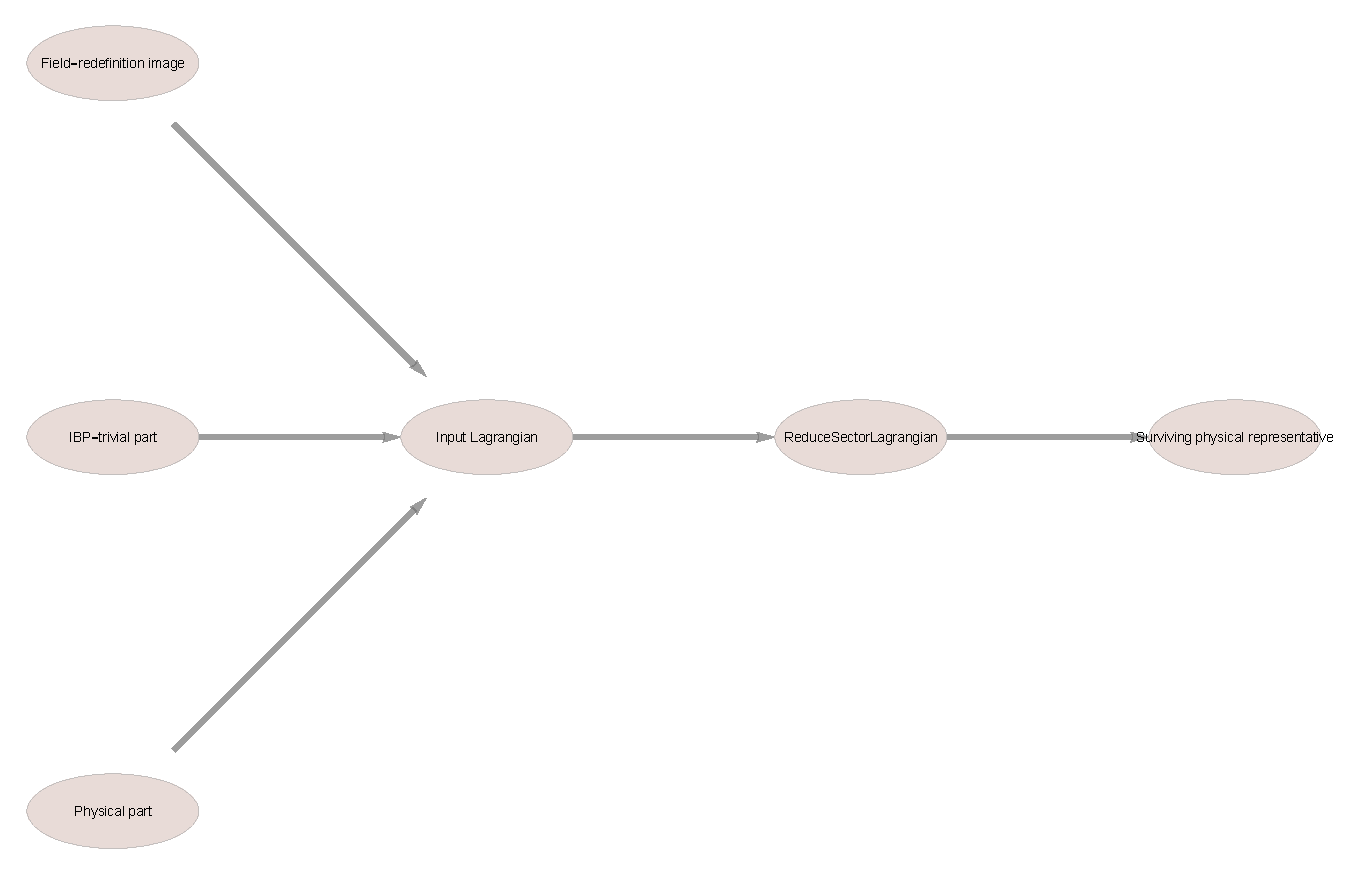
\includegraphics[width=0.82\textwidth,height=0.30\textheight,keepaspectratio]{paper_assets/worked_example_pipeline.pdf}
  \caption{Structure of the worked example.}
  \label{fig:worked_example_pipeline}
\end{figure}

\section{Mathematical expectation}

The quotient logic is immediate:
\begin{equation}
  [\Lag_{\IBP}] = 0
  \quad\text{in}\quad
  \Qspace{3}{2},
  \label{eq:worked_ibp_zero}
\end{equation}
and
\begin{equation}
  [\Lag_{\FieldRed}] = 0
  \quad\text{in}\quad
  \Pspace{3}{2}.
  \label{eq:worked_redef_zero}
\end{equation}
Therefore
\begin{equation}
  [\Lag_{\mathrm{in}}]
  =
  [\Lag_{\Phys}] + 4[0] + [0]
  =
  [\Lag_{\Phys}].
  \label{eq:worked_expected_class}
\end{equation}
Thus the reduced answer must be nonzero and must coincide with the chosen physical representative.

\section{Coordinate-level reduction}

Projecting the full input into the \((3,2)\) IBP basis gives
\begin{equation}
  \bm{q}_{\IBP}^{\mathrm{in}}
  =
  \{2,7,-24,61,-66,-3,5,-54,73,10,10,-10,-19,7\}.
  \label{eq:worked_input_ibp_coords}
\end{equation}
After subtracting the field-redefinition image, the reduced IBP coordinates are
\begin{equation}
  \bm{q}_{\IBP}^{\mathrm{red}}
  =
  \{2,0,0,0,0,-3,0,0,0,0,0,0,0,0\}.
  \label{eq:worked_reduced_ibp_coords}
\end{equation}
Hence the image component itself is
\begin{equation}
  \bm{q}_{\IBP}^{\FieldRed}
  =
  \bm{q}_{\IBP}^{\mathrm{in}} - \bm{q}_{\IBP}^{\mathrm{red}}
  =
  \{0,7,-24,61,-66,0,5,-54,73,10,10,-10,-19,7\}.
  \label{eq:worked_image_coords}
\end{equation}
By construction, \eqref{eq:worked_image_coords} is generated from the image coefficients
\begin{equation}
  \bm{\alpha}_{\FieldRed}
  =
  \{5,-7,11,-13\}.
  \label{eq:worked_recovered_alpha}
\end{equation}
Finally, the physical coordinates are
\begin{equation}
  \bm{q}_{\Phys}^{\mathrm{in}}
  =
  \{2,-3,0,0,0,0,0,0,0,0\},
  \label{eq:worked_final_phys_coords}
\end{equation}
which agree exactly with \eqref{eq:worked_phys_coords}.

\section{Reduced representative}

The final reduced expression returned by the code is
\begin{lstlisting}[style=mma]
2*h[a, b]*PD[-a][h[c, d]]*PD[-b][h[-c, -d]]
- 3*h[a, b]*PD[-b][h[-a, c]]*PD[-d][h[-c, d]]
\end{lstlisting}
which matches \(\Lag_{\Phys}\) term by term.
This is the desired nontrivial example:
both the IBP-trivial and field-redefinition-trivial pieces are removed,
but the result is not zero because the input contained a genuine physical component.

\section{Mathematica commands used}

For completeness, the example was generated by
\begin{lstlisting}[style=mma]
sec = ComputeSectorData[3, 2, Sequence @@ opts];
physCoeffs = ReplacePart[ConstantArray[0, sec["PhysicalCount"]], {1 -> 2, 2 -> -3}];
physExpr = canonExpr @ LinearCombination[physCoeffs, sec["PhysicalBasis"]];
ibpExpr = sec["IBPRelationExpressions"][[1]];
redefCoeffs = {5, -7, 11, -13};
redefExpr = canonExpr @ Total[MapThread[Times, {redefCoeffs, sec["RedefShiftImages"]}]];
lag = canonExpr @ Expand[physExpr + 4 ibpExpr + redefExpr];
red = ReduceSectorLagrangian[lag, 3, 2, Sequence @@ opts];
\end{lstlisting}

\chapter{Reproduction, Files, and Further Work}

The principal files relevant to the current report are:
\begin{itemize}
\item \toolkit\ --- the implementation;
\item \validationdata\ --- machine-readable validation output for the \((3,2)\) and \((3,4)\) image tests;
\item \reportdata\ --- machine-readable data used by the notebook-style comprehensive report;
\item \texttt{paper\_assets/} --- the vector figures used by the present paper-style report;
\item \texttt{graviton\_basis\_toolkit\_paper\_report.tex} --- the present LaTeX source;
\item \texttt{graviton\_basis\_toolkit\_paper\_report.pdf} --- the compiled PDF.
\end{itemize}

If the implementation changes, the recommended update order is:
\begin{enumerate}[label=\arabic*.]
\item rerun the sector validation script;
\item regenerate the comprehensive report data;
\item regenerate the paper assets;
\item recompile the paper report.
\end{enumerate}

There are several natural directions for future refinement:
\begin{enumerate}[label=\alph*.]
\item add a gauge-invariance layer on top of the current quotient spaces;
\item extend the sector construction to multi-field theories;
\item add appendices with full basis listings in selected sectors;
\item derive curvature-based representations of the surviving four-derivative quadratic classes.
\end{enumerate}

\end{document}
